% \VignetteIndexEntry{Smoothing discrete data (I) - smooth.discrete()}
% \VignetteDepends{mhsmm}
% \VignetteKeyword{Hidden Markov Model}

\documentclass{article}
\usepackage{a4wide}
\usepackage[T1]{fontenc}
\usepackage[latin1]{inputenc}

\title{Smoothing discrete data (I)\\ -- using the \texttt{smooth.discrete()} function in the
  \texttt{mhsmm} package}
\author{S{\o}ren H{\o}jsgaard and Jared O'Connell}

\def\code#1{\texttt{#1}}

\usepackage{Sweave}
\begin{document}

 
\setkeys{Gin}{width=0.5\textwidth,height=2in}
\renewenvironment{Schunk}{\linespread{.85}\small}{}

\maketitle

\parindent0pt\parskip5pt

\tableofcontents

\begin{Schunk}
\begin{Soutput}
hsmm shared library loaded
\end{Soutput}
\end{Schunk}


\section{Introduction}


The \verb'smooth.discrete()' function provides a simple smoothing of a
time series of discrete values measured at equidistant times.
Under the hood of  \verb'smooth.discrete()' is a hidden Markov model.

More details -- and an additional example -- is provided in the
vignette ``Smoothing discrete data (II)''

\section{Using \texttt{smooth.discrete()}}

For example consider the data:
\begin{Schunk}
\begin{Sinput}
> y1 <- c(1, 1, 1, 1, 2, 1, 1, NA, 1, 1, 2, 1, 1, 1, 2, 1, 1, 1, 
+     1, 1, 2, 2, 2, 2, 1, 2, 2, 2, 1, 2, 2, 2, 1, 1, 1, 1, 1, 
+     1, 1, 1, 2, 2, 2, 1, 1)
\end{Sinput}
\end{Schunk}

Calling \verb'smooth.discrete()' on these data gives 
\begin{Schunk}
\begin{Sinput}
> obj <- smooth.discrete(y1)
\end{Sinput}
\begin{Soutput}
A 'smoothDiscrete' object
List of 4
 $ s      : num [1:45] 1 1 1 1 1 1 1 1 1 1 ...
 $ model  :List of 9
  ..- attr(*, "class")= chr "hmm"
 $ data   :List of 3
 $ initial:List of 3
 - attr(*, "class")= chr "smoothDiscrete"
NULL
\end{Soutput}
\end{Schunk}

The \verb's' slot of the object contains the smoothed values. We
illustrate the results in Figure~\ref{fig:smooth1}.

\begin{Schunk}
\begin{Sinput}
> plot(y1, ylim = c(0.8, 2))
> addStates(obj$s)
\end{Sinput}
\end{Schunk}

\begin{figure}[h]
  \centering
  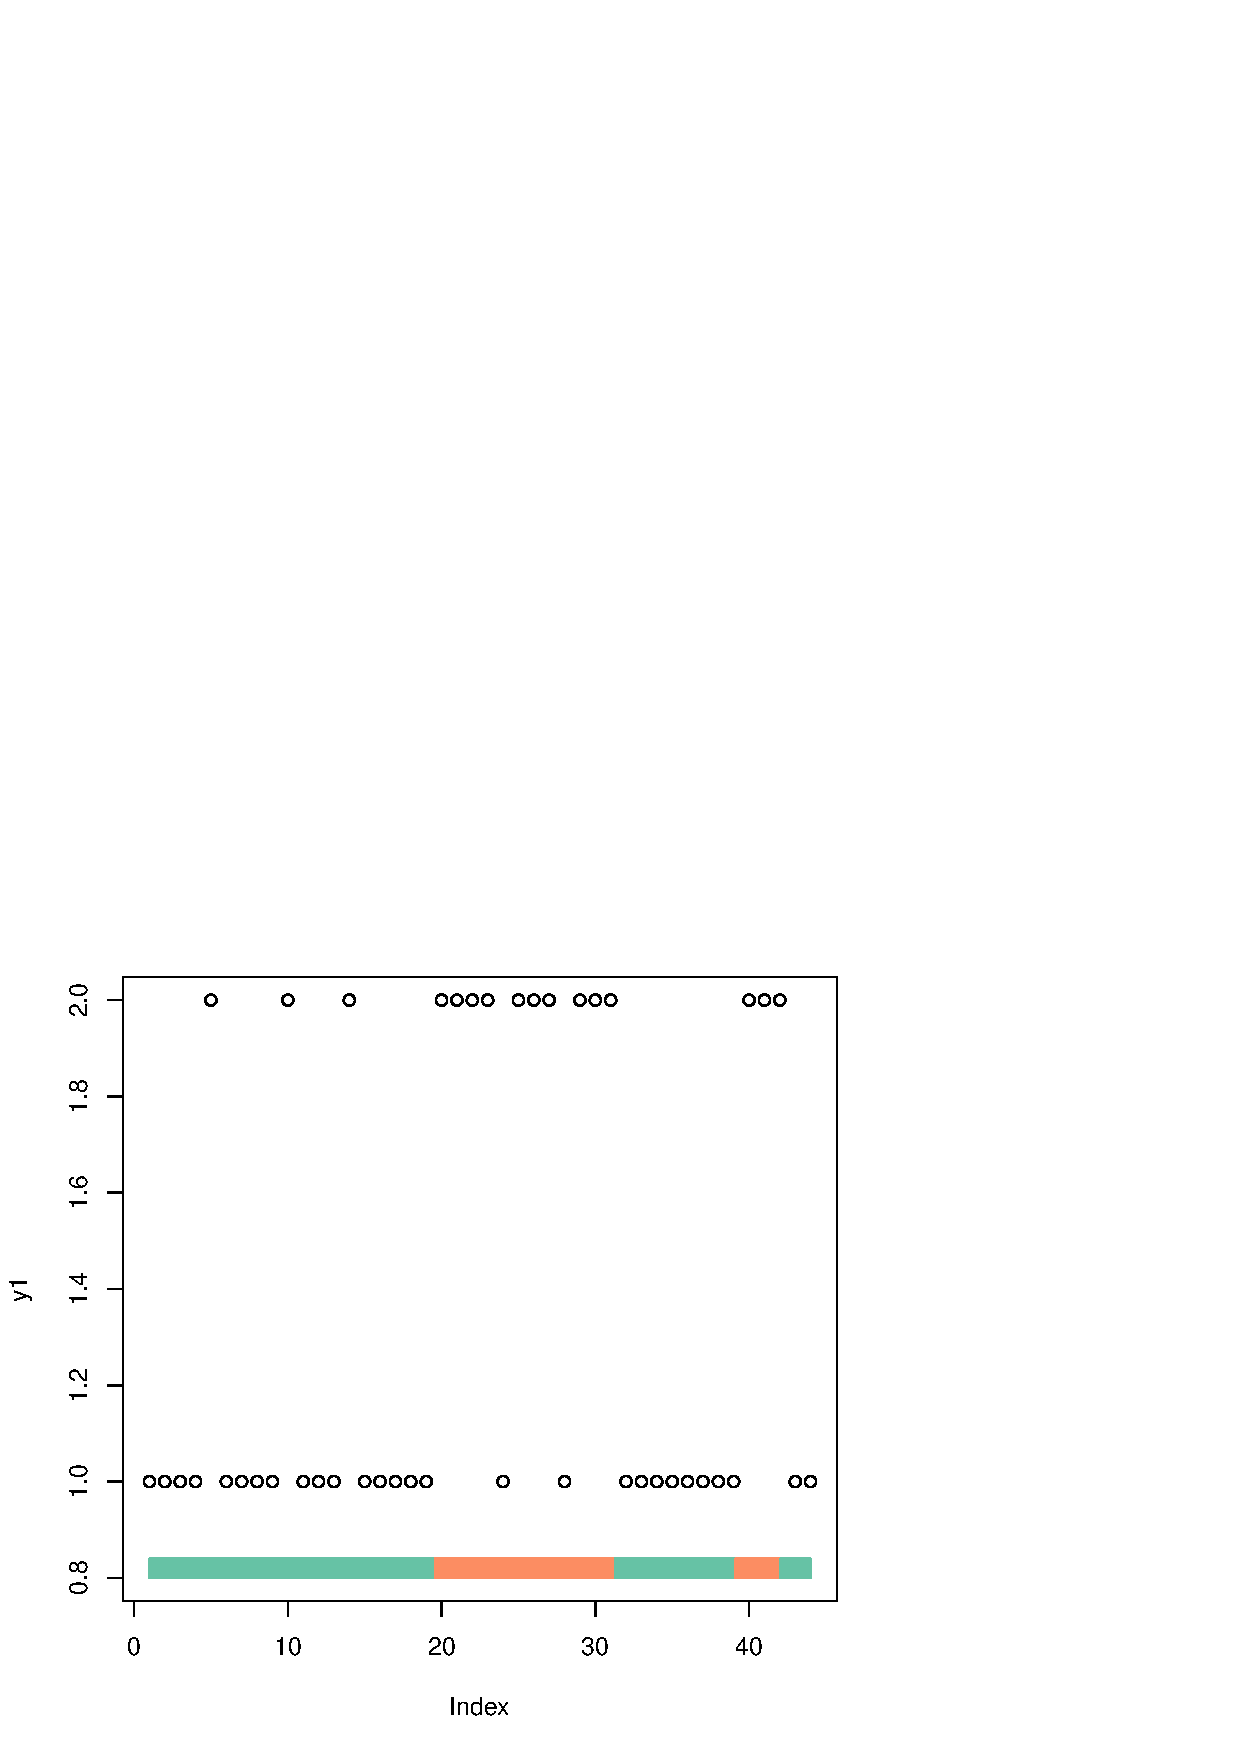
\includegraphics{fig/smooth-smooth1}
  \caption{Observed and smoothed discrete time time series.}
  \label{fig:smooth1}
\end{figure}

The smoothed sequence of states is by default the jointly most likely
sequence of states as obtained by the Viterbi algorithm.

A smooth of a new time series is produced as
\begin{Schunk}
\begin{Sinput}
> y2 <- c(1, 1, 1, 1, 2, 2, 2, 1, 1, 2, 1, 1, 1, 2, 1, 1, 1, 1, 
+     1, 2, 2, 2, NA, 1, 1, 1, 2, 2, 1, 2, 2, 2)
> predict(obj, x = y2)
\end{Sinput}
\begin{Soutput}
$s
 [1] 1 1 1 1 1 1 1 1 1 1 1 1 1 1 1 1 1 1 1 2 2 2 2 2 2 2 2 2 2 2 2 2

$x
 [1]  1  1  1  1  2  2  2  1  1  2  1  1  1  2  1  1  1  1  1  2  2  2 NA  1  1
[26]  1  2  2  1  2  2  2

$N
[1] 32

$loglik
[1] -24.53755

attr(,"class")
[1] "hsmm.data"
\end{Soutput}
\end{Schunk}

Here the smoothed values are in the \verb's' slot.
Again, the sequence is by default the jointly most likely
sequence of states. 


The estimated parameters are:
\begin{Schunk}
\begin{Sinput}
> summary(obj)
\end{Sinput}
\begin{Soutput}
init: 
 1 0 

transition:
      [,1]  [,2]
[1,] 0.920 0.080
[2,] 0.136 0.864

emission:
$pmf
          [,1]      [,2]
[1,] 0.7925235 0.2147958
[2,] 0.3418576 0.6443388
\end{Soutput}
\end{Schunk}


\section{The arguments to \texttt{smooth.discrete()}}
\label{sec:xxx}



The arguments of \verb'smooth.discrete()' are
\begin{Schunk}
\begin{Sinput}
> args(smooth.discrete)
\end{Sinput}
\begin{Soutput}
function (y, init = NULL, trans = NULL, parms.emission = 0.5, 
    method = "viterbi", details = 0, ...) 
NULL
\end{Soutput}
\end{Schunk}

\begin{itemize}

\item \code{init} is a vector of initial probabilities for the Markov
chain. 
If \code{init=NULL} then the initial distribution is taken to be
the relative frequencies in data, that is
\begin{Schunk}
\begin{Sinput}
> table(y1)/sum(table(y1))
\end{Sinput}
\begin{Soutput}
y1
        1         2 
0.6363636 0.3636364 
\end{Soutput}
\end{Schunk}

\item \code{trans} is the transition matrix for the Markov chain.
If \code{trans=NULL} then the transition matrix is derived from data as:
\begin{Schunk}
\begin{Sinput}
> ttt <- table(y1[-length(y1)], y1[-1])
> ttt
\end{Sinput}
\begin{Soutput}
     1  2
  1 19  7
  2  7  9
\end{Soutput}
\begin{Sinput}
> sweep(ttt, 1, rowSums(ttt), "/")
\end{Sinput}
\begin{Soutput}
            1         2
  1 0.7307692 0.2692308
  2 0.4375000 0.5625000
\end{Soutput}
\end{Schunk}

If \code{trans} is a vector (of numbers smaller than $1$) then these
are taken to be the diagonal of the transition matrix and the
off--diagonal elements are then, within each row, taken to be
identical so that the rows sum to $1$. Elements of \code{trans} are
recycled so as to make the dimensions match. Under the hood, the
matrix is created as, for example:

\begin{Schunk}
\begin{Sinput}
> createTransition(c(0.8, 0.9), 2)
\end{Sinput}
\begin{Soutput}
     [,1] [,2]
[1,]  0.8  0.2
[2,]  0.1  0.9
\end{Soutput}
\end{Schunk}

\item \code{parms.emission} is a matrix describing the conditional
  probabilities of the observed states given the latent states. If
  \code{parms.emission} is a vector then the matrix is created
  following the same scheme as for the transition matrix described
  above. 


\item The \verb'method' argument is either
\verb'"viterbi"' (which produces the jointly most likely
sequence of states). The alternative method is \verb'smoothed' which
produces the individually most likely states. 


\item The dotted arguments are
passed on the the \verb'hmmfit' function. For example, one may specify
\code{lock.transition=TRUE} in which case the transition matrix is not
estimated from data.

\end{itemize}






\end{document}





